\chapter{Empirical evaluation of compression algorithms}
In this chapter, we compare different compression algorithms in terms of compression ratio using both real
and generated time series data. The compression algorithms that we have chosen are Gorilla, LZ4,
Deflate and Zstandard. By doing this we want to evaluate whether compression algorithms specifically
targeted to time series are better than general-purpose algorithms.

\section{Datasets}
For these benchmarks, we have used three different datasets. The first dataset was generated from the
Time Series Benchmark Suite, a command-line tool written by TimescaleDB \cite{timescale_2019_timescaletsbs} that makes
easy to generate realistic time-series data to benchmark different time series databases.
The second dataset was created by using Dynatrace. Dynatrace is a Software Intelligence platform with a strong
emphasis on application performance monitoring. The datasets consist of metrics gathered from
different hosts running a wide range of applications under different loads.
The third dataset was provided by the New York Taxi and Limousine Commission (TLC), and it consists
of records representing taxi trips, including information such as duration of the trip, amount
charged, tip amount \cite{tlc2019_dataset}.

\subsection{Generating devops data}
As we have mentioned above, we have used the TimeSeries Benchmark Suite to generate fake DevOps data.
This utility allows to specify which use case to simulate data for, which time interval between each data points
to use, the starting timestamp and the ending timestamp, how many hosts to simulate.
We have decided to generate data points every minute, for a single host and for 5 different time intervals:
2 hours, 4 hours, 8 hours, 16 hours and 48 hours. For each of these intervals, we generate 50 different time-series.

\subsection{Collecting Dynatrace Data}
Dynatrace provides a REST API to retrieve metrics it collects \cite{a2013_metrics}.
We have used this API to retrieve data of several hosts which were monitored in one of the demo environment
Dynatrace uses for testing purposes.
The metrics we have chosen to collect are the following:
\begin{itemize}
    \item Host CPU Usage: Percentage of overall CPU usage
    \item Host CPU System: Percentage of CPU time used by the kernel
    \item Host CPU User: Percentage of CPU time used by userspace processes
    \item Host CPU Io Wait: Percentage of CPU time spent waiting for input/output operations
    \item Host Memory Used: Percentage of memory used
    \item Host Memory Usage: Memory usage in bytes
    \item Host Disk Read Time: Disk read time in milliseconds
    \item Host Disk Write Time: Disk write time in milliseconds
\end{itemize}

\subsection{Taxi Data}
The taxi data set was provided by the New York Taxi and Limousine Commission. For each month of the year,
the TLC provide a data set for the two different taxi companies running in New York (green and yellow)
and for limousines. We have decided to take into account only yellow taxi data for one month.
Moreover, to make in-memory compression feasible, we have dropped the last 3 million records from the
dataset. Additionally, all the columns containing string data were removed since they are not handled
by the Gorilla algorithm.

\section{Compressing data}
The metric which we are interested in these benchmarks is the compression ratio, while we do not evaluate compression speed
as this is dependent on the specifics algorithms implementations.
We have created a Java program that reads data from the input stream and returns the compression ratio
achieved by the algorithm selected. We decided to use Java because we could easily find implementations for
all the algorithms listed above.
The program requires to specify the format of the dataset provided in the standard input and the
algorithm to use for compression, as the following listing illustrates.
\lstset{
    basicstyle=\small,
    stringstyle=\ttfamily
}
\begin{lstlisting}[language=bash]
  $ ./gradlew shadowJar
  $ java -jar
  TimeseriesCompressionBenchmarks-all.jar [format] [algorithm]
\end{lstlisting}
Gorilla compression does not work on byte data. It needs instead pairs of values and timestamps.
For this reason, we parse each time-series file to obtain a TimeSeries object.
This object contains a key and a list of value-timestamp pairs.  
We pass this TimeSeries object to a compressor, which is an interface responsible for returning a compressed version of the time-series.
In the case of Gorilla compression, we have implemented this interface by iterating through all
the data points, pushing those to the Gorilla compression library, and returning the compressed
version of the time-series, which is a long array in the case of the Gorilla Compression library we are using.
With the other compression algorithms, we could serialize the TimeSeries
object to a byte array, compress it, and get back a compressed byte array. 
The way we compute the compression ratio is by dividing the number of bytes representing the serialized
time-series object, divided by the number of bytes of the serialized compressed time-series.
The code is available on github \cite{dovidio_2019_dovidiotscompressionthesis}.
For gorilla compression, we have used an open source java implementation of the algorithm
\cite{burmanm_2018_burmanmgorillatsc}. Deflate, on the other hand, is already present in the the package
\textit{java.util.zip}, using the zlib library under the hood \cite{a2019_deflater}.
For LZ4 and ZStandard we have used open source implementations \cite{lz4_2019_lz4lz4java}\cite{luben_2015_lubenzstdjni}.

\section{Results}
\subsection{Generated data}
Figure~\ref{devops_lossless_compression} illustrates the result of applying different compression algorithms
with generated data. It clearly shows how Gorilla (mean = 13.349707, standard deviation = 1.597951), is outperforming the other
lossless compression algorithms.
It is also interesting to notice how ZStandard (mean = 3.580531, standard deviation = 0.319150) and Deflate
(mean = 3.224456, standard deviation = 0.240666)
performs similarly, while LZ4 (mean = 2.364515, standard deviation = 0.135801) has
consistently the worst compression ratio, as one might have predicted given that it was engineered to optimize compression speed rather
than compression ratio.

\begin{figure}[!htbp]
\begin{center}
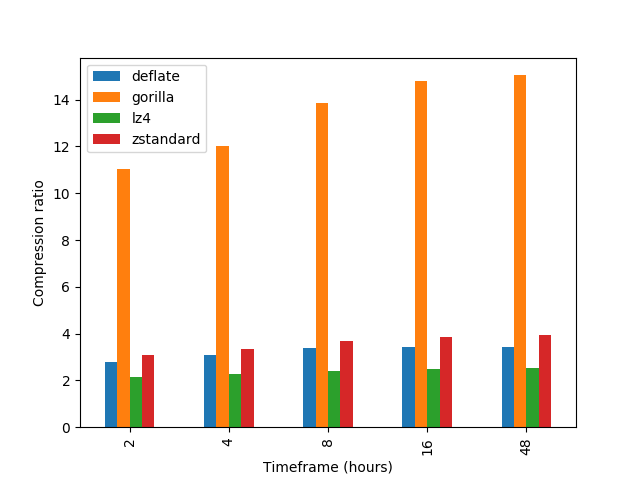
\includegraphics[width=300pt]{devops_bar_chart}
\caption[compression]{Generated data compressed with Gorilla, Deflate, ZStandard, LZ4.
Higher values indicates higher compression ratios.}
\label{devops_lossless_compression}
\end{center}
\end{figure}

\subsection{Dynatrace Data}
Results of the different compression algorithms applied to real-word series data are shown in
Figure~\ref{dynatrace_compression}. The results are similar to what we have seen for generated data,
with Gorilla outperforming general purposes algorithm across all metrics.

\begin{figure}[!htbp]
\begin{center}
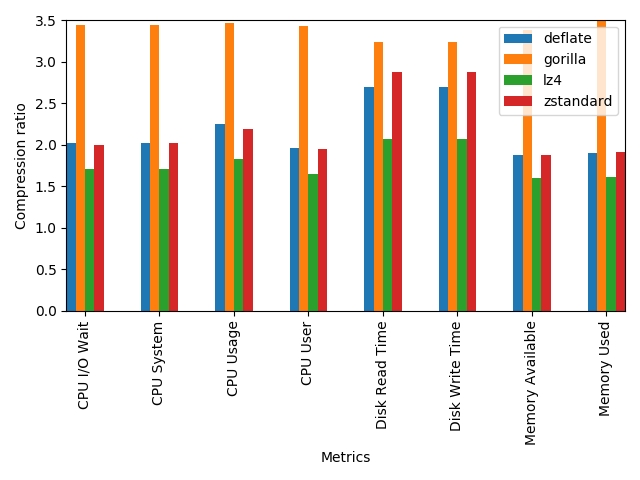
\includegraphics[width=300pt]{dynatrace_bar_chart}
\caption[compression]{Real world data collected by Dynatrace compressed with Gorilla, Deflate, ZStandard, LZ4.
Higher values indicates higher compression ratios.}
\label{dynatrace_compression}
\end{center}
\end{figure}

\subsection{Taxi Data}
For taxi data, we have decided to transform the data in a column format.
Since each record contains 15 columns, this means that we have transformed data in 15 time series,
ordered by pick up time.
Each time series data point represent a specific value for a specific taxi trip.
The time interval between each data point is not regular as in the previous data sets, for this
reason Gorilla delta of delta timestamp compression is likely to not yield good compression
ratios.
As Figure~\ref{taxi_bar_chart} shows, Gorilla compression does not perform well for this use case.
Its performance is on par with LZ4, while both Deflate and ZStandard achieve better compression ratio.

\begin{figure}[!htbp]
\begin{center}
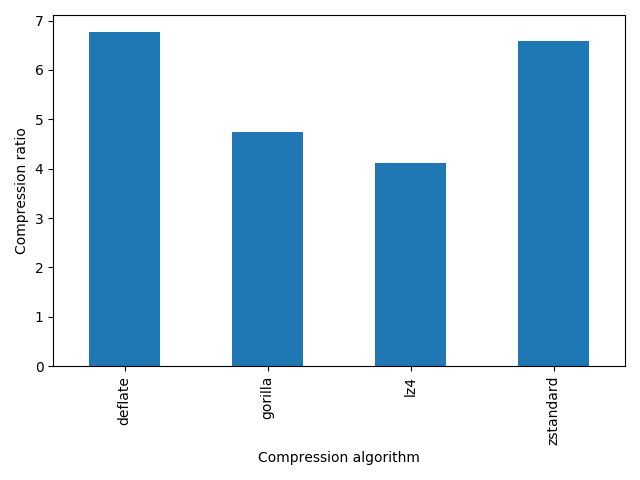
\includegraphics[width=300pt]{taxi_bar_chart}
\caption[compression]{Taxi Data compressed with Gorilla, Deflate, ZStandard, LZ4.
Higher values indicates higher compression ratios.}
\label{taxi_bar_chart}
\end{center}
\end{figure}